\documentclass{article}
\usepackage{amsmath, sfmath, multicol, tkz-euclide, array, enumerate, tcolorbox, tabularray}
\renewcommand{\familydefault}{\sfdefault}
\setlength{\parindent}{0cm}
\pagestyle{empty}
\usepackage[left=1in, top=0.5in, right=1in, bottom=0.5in]{geometry}
\tikzset{>=stealth, label style/.append style={font=\footnotesize}}
\tcbset{colback=white}

\newcounter{example}[section]
\newenvironment{example}[1][]{\refstepcounter{example}\par\medskip
   {\color{red}\textbf{Example~\theexample. #1}}}{\medskip}

\begin{document}

\section*{Trigonometry and Area}

\begin{tcolorbox}[colframe=orange!70!white, coltitle=black, title=\textbf{Today I Can}]
\begin{enumerate}
    \item Find areas of triangles and regular polygons using trigonometry.
\end{enumerate}
\end{tcolorbox}
\smallskip 

\begin{example}
Find the area of each.
\begin{multicols}{2}
\begin{enumerate}[(a)]
    \item \mbox{} \newline 
    \item \mbox{} \newline 
\end{enumerate}
\end{multicols}
\begin{minipage}{0.6\textwidth}
    \begin{tikzpicture}[scale=0.8, rotate=50]
    \tkzDefPoints{0/0/O, 2/0/A}
    \tkzDefShiftPoint[O](40:2){B}
    \tkzDefShiftPoint[O](80:2){C}
    \tkzDefShiftPoint[O](120:2){D}
    \tkzDefShiftPoint[O](160:2){E}
    \tkzDefShiftPoint[O](200:2){F}
    \tkzDefShiftPoint[O](240:2){G}
    \tkzDefShiftPoint[O](280:2){H}
    \tkzDefShiftPoint[O](320:2){I}
    \tkzDrawPolygon(A,B,C,D,E,F,G,H,I)
    \tkzLabelSegment[right](H,I){\footnotesize 10 cm}
    \end{tikzpicture}
\end{minipage}
\begin{minipage}{0.3\textwidth}
    \begin{tikzpicture}[scale=0.75]
    \tkzDefPoints{0/0/O, 0/2/A}
    \tkzDefShiftPoint[O](162:2){B}
    \tkzDefShiftPoint[O](234:2){C}
    \tkzDefShiftPoint[O](306:2){D}
    \tkzDefShiftPoint[O](378:2){E}
    \tkzDrawPolygon(A,B,C,D,E)
    \tkzDefMidPoint(C,D)
    \tkzGetPoint{F}
    \tkzLabelSegment[below](D,C){\footnotesize 4 in}
    \end{tikzpicture}
\end{minipage}
\end{example}

\vspace{2in}

\begin{example}
A stop sign is a regular octagon. The standard size has a 16.2 in radius. What is the area of the stop sign to the nearest square inch? \newline 

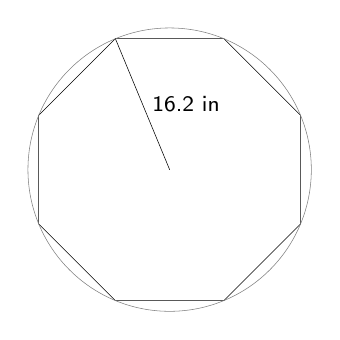
\begin{tikzpicture}[scale=0.9, rotate=22.5]
\tkzDefPoints{0/0/O, 2/0/A}
\tkzDefShiftPoint[O](45:2){B}
\tkzDefShiftPoint[O](90:2){C}
\tkzDefShiftPoint[O](135:2){D}
\tkzDefShiftPoint[O](180:2){E}
\tkzDefShiftPoint[O](225:2){F}
\tkzDefShiftPoint[O](270:2){G}
\tkzDefShiftPoint[O](315:2){H}
\tkzDrawPolygon(A,B,C,D,E,F,G,H)
\tkzDrawCircle(O,A)
\tkzDrawSegment(O,C)
\tkzLabelSegment[midway, right](O,C){\footnotesize 16.2 in}
\end{tikzpicture}
\end{example}

\newpage 

\begin{tcolorbox}[colframe=black!20!white, opacitybacktitle=0.1, coltitle=black, title=\textbf{Area of a SAS Triangle}]
\begin{minipage}{0.3\textwidth}
\begin{itemize}
    \item Area = $\frac{1}{2}bc\times \sin A$
\end{itemize}
\end{minipage}
\begin{minipage}{0.4\textwidth}
    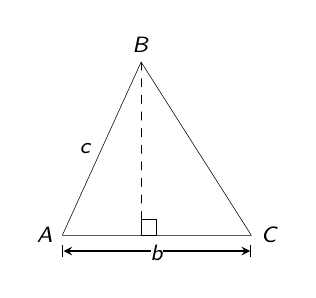
\begin{tikzpicture}[scale=0.8]
    \tkzDefPoints{0/0/A, 3/0/C, 1.25/2.75/B}
    \tkzDrawPolygon(A,B,C)
    \tkzLabelPoints[left](A)
    \tkzLabelPoints[right](C)
    \tkzLabelPoints[above](B)
    \tkzDefLine[orthogonal = through B](A,C)
    \tkzGetPoint{D}
    \tkzInterLL(B,D)(A,C)
    \tkzGetPoint{E}
    \tkzDrawSegment[dashed](B,E)
    \tkzMarkRightAngle(C,E,B)
    \tkzLabelSegment[left](A,B){$c$}
    \tkzLabelSegment[below](A,C){$b$}
    \draw [->|, >=stealth] (1.4,-0.25) -- (0,-0.25);
    \draw [->|, >=stealth] (1.6,-0.25) -- (3,-0.25);
    \end{tikzpicture}
\end{minipage}
\end{tcolorbox}

\begin{example}
Find the area of each triangle. Round your answers to 2 decimal places.
\begin{multicols}{2}
\begin{enumerate}[(a)]
    \item \mbox{} \newline 
    \item \mbox{} \newline 
\end{enumerate}
\end{multicols}
\begin{minipage}{0.5\textwidth}
    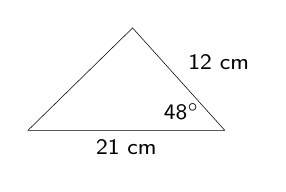
\begin{tikzpicture}
    \tkzDefPoints{0/0/A, 2.5/0/B}
    \tkzDefShiftPoint[B](132:1.75){C}
    \tkzDrawPolygon(A,B,C)
    \tkzLabelAngle[pos=0.6](C,B,A){\footnotesize $48^\circ$}
    \tkzLabelSegment[below](A,B){\footnotesize 21 cm}
    \tkzLabelSegment[above right](B,C){\footnotesize 12 cm}
    \end{tikzpicture}
\end{minipage}
\begin{minipage}{0.4\textwidth}
    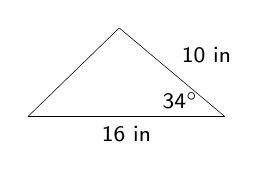
\begin{tikzpicture}
    \tkzDefPoints{0/0/A, 2.5/0/B}
    \tkzDefShiftPoint[B](140:1.75){C}
    \tkzDrawPolygon(A,B,C)
    \tkzLabelAngle[pos=0.6](C,B,A){\footnotesize $34^\circ$}
    \tkzLabelSegment[below](A,B){\footnotesize 16 in}
    \tkzLabelSegment[above right](B,C){\footnotesize 10 in}
    \end{tikzpicture}
\end{minipage}
\end{example}

\vspace{1.5in}

\begin{example}
A tabletop has the shape of a regular decagon with a radius of 9.5 in. What is the area of the tabletop to the nearest square inch?
\end{example}

\end{document}
